\documentclass{article}
\usepackage[]{graphicx}
\graphicspath{ {./images/} }
\usepackage[]{color}
%\usepackage{hyperref}

\usepackage[colorlinks=true,linkcolor=blue]{hyperref}

\usepackage{listings}

\definecolor{dkgreen}{rgb}{0,0.6,0}
\definecolor{gray}{rgb}{0.5,0.5,0.5}
\definecolor{mauve}{rgb}{0.58,0,0.82}

\lstset{frame=tb,
  language=bash,
  aboveskip=3mm,
  belowskip=3mm,
  showstringspaces=false,
  columns=flexible,
  basicstyle={\small\ttfamily},
  numbers=none,
  numberstyle=\tiny\color{gray},
  keywordstyle=\color{blue},
  commentstyle=\color{dkgreen},
  stringstyle=\color{red},
  breaklines=true,
  breakatwhitespace=true,
  tabsize=3
}

\usepackage{enumitem}% http://ctan.org/pkg/enumitem

% maxwidth is the original width if it is less than linewidth
% otherwise use linewidth (to make sure the graphics do not exceed the margin)
\makeatletter
\def\maxwidth{ %
  \ifdim\Gin@nat@width>\linewidth
    \linewidth
  \else
    \Gin@nat@width
  \fi
}
\makeatother

\definecolor{fgcolor}{rgb}{0.345, 0.345, 0.345}
\newcommand{\hlnum}[1]{\textcolor[rgb]{0.686,0.059,0.569}{#1}}%
\newcommand{\hlstr}[1]{\textcolor[rgb]{0.192,0.494,0.8}{#1}}%
\newcommand{\hlcom}[1]{\textcolor[rgb]{0.678,0.584,0.686}{\textit{#1}}}%
\newcommand{\hlopt}[1]{\textcolor[rgb]{0,0,0}{#1}}%
\newcommand{\hlstd}[1]{\textcolor[rgb]{0.345,0.345,0.345}{#1}}%
\newcommand{\hlkwa}[1]{\textcolor[rgb]{0.161,0.373,0.58}{\textbf{#1}}}%
\newcommand{\hlkwb}[1]{\textcolor[rgb]{0.69,0.353,0.396}{#1}}%
\newcommand{\hlkwc}[1]{\textcolor[rgb]{0.333,0.667,0.333}{#1}}%
\newcommand{\hlkwd}[1]{\textcolor[rgb]{0.737,0.353,0.396}{\textbf{#1}}}%
\let\hlipl\hlkwb

\usepackage{framed}
\makeatletter
\newenvironment{kframe}{%
 \def\at@end@of@kframe{}%
 \ifinner\ifhmode%
  \def\at@end@of@kframe{\end{minipage}}%
  \begin{minipage}{\columnwidth}%
 \fi\fi%
 \def\FrameCommand##1{\hskip\@totalleftmargin \hskip-\fboxsep
 \colorbox{shadecolor}{##1}\hskip-\fboxsep
     % There is no \\@totalrightmargin, so:
     \hskip-\linewidth \hskip-\@totalleftmargin \hskip\columnwidth}%
 \MakeFramed {\advance\hsize-\width
   \@totalleftmargin\z@ \linewidth\hsize
   \@setminipage}}%
 {\par\unskip\endMakeFramed%
 \at@end@of@kframe}
\makeatother

\definecolor{shadecolor}{rgb}{.97, .97, .97}
\definecolor{messagecolor}{rgb}{0, 0, 0}
\definecolor{warningcolor}{rgb}{1, 0, 1}
\definecolor{errorcolor}{rgb}{1, 0, 0}
\newenvironment{knitrout}{}{} % an empty environment to be redefined in TeX

\usepackage{alltt}

\title{Getting Started with Raspberry Pi}
\IfFileExists{upquote.sty}{\usepackage{upquote}}{}


\author{Kyle McCarty and Marc Los Huertos\footnote{Acknowledgments: Summer research students, Anna Burns and Alision Joseph contributed to these documents.}}
\title{Getting Started with Raspberry Pi}

\begin{document}

\maketitle

\newpage

\tableofcontents

\newpage

\section{Introduction}

\subsection{What is a Raspberry Pi?}

The Raspberry Pi is an tiny computer, that includes a microprocessor, a bit of memory, a slot for an SD card, input/output (I/O) ports, e.g. HDMI, USB, headphone, camera, and some general purpose input/output (GPIO) pins for various types of electrical connectors.

\subsection{Why use the Raspberry Pi?}

Generally, Raspberry Pis draw considerably less power than regular computers, are a lot smaller, and are relatively cost-effective. In addition, the GPIO pins allow for connecting and controlling various types of electrical components, such as LEDs and sensors. Raspberry Pis are very flexible devices. They can be used for personal computers, home survaillance systems, weather stations, adblockers for your home network, retro gaming machines, as an AI assistant, and so much more! In this class, we'll be using it as an environmental monitoring device.

\subsection{Packaging List}

Here are the things you will have to work with: 

\begin{enumerate}[noitemsep]
  \item Raspberry Pi Zero W board
  \item Case
  \item 2.5A power supply
  \item HDMI to mini-HDMI adapter
  \item USB to micro-USB adapter
  \item Header pin diagram
  \item PMS5003 Particulate Sampler
  \item BME280 Temperature, Humidity, and Pressure sensor
  \item Cables
  \item micro-SD card
\end{enumerate}

\subsubsection{Other items}

\begin{enumerate}[noitemsep]
  \item SD card
  \item SD card to USB adapter
  \item USB multiport adapter
  \item Breadboard
  \item Wires
  \item Line level converter (LLC)
  \item MCP3008
  \item various MQ-sensors

\end{enumerate}

\subsection{Preloaded Micro-SD Card}

Here's what we have done to prepare for class:

\begin{enumerate}
  \item Used ``Raspberry Pi Imager'' to image micro-SD card (\url{https://www.raspberrypi.org/downloads/}) (Figure~\label{fig:pi_imager}).
  
\begin{figure}
\centering
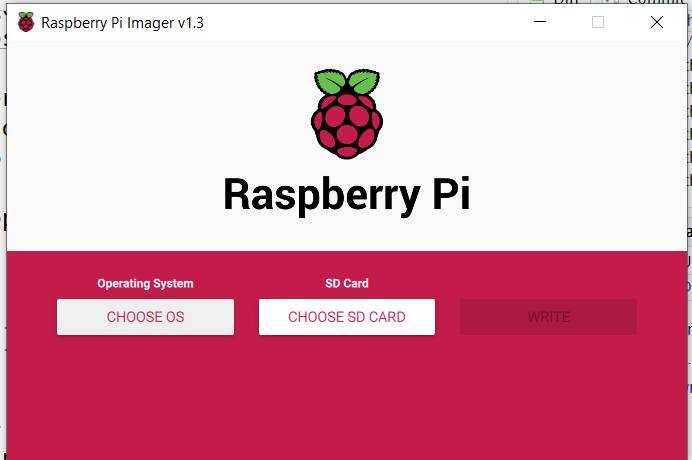
\includegraphics[width=1.00\textwidth]{1_Pi_Imager}
%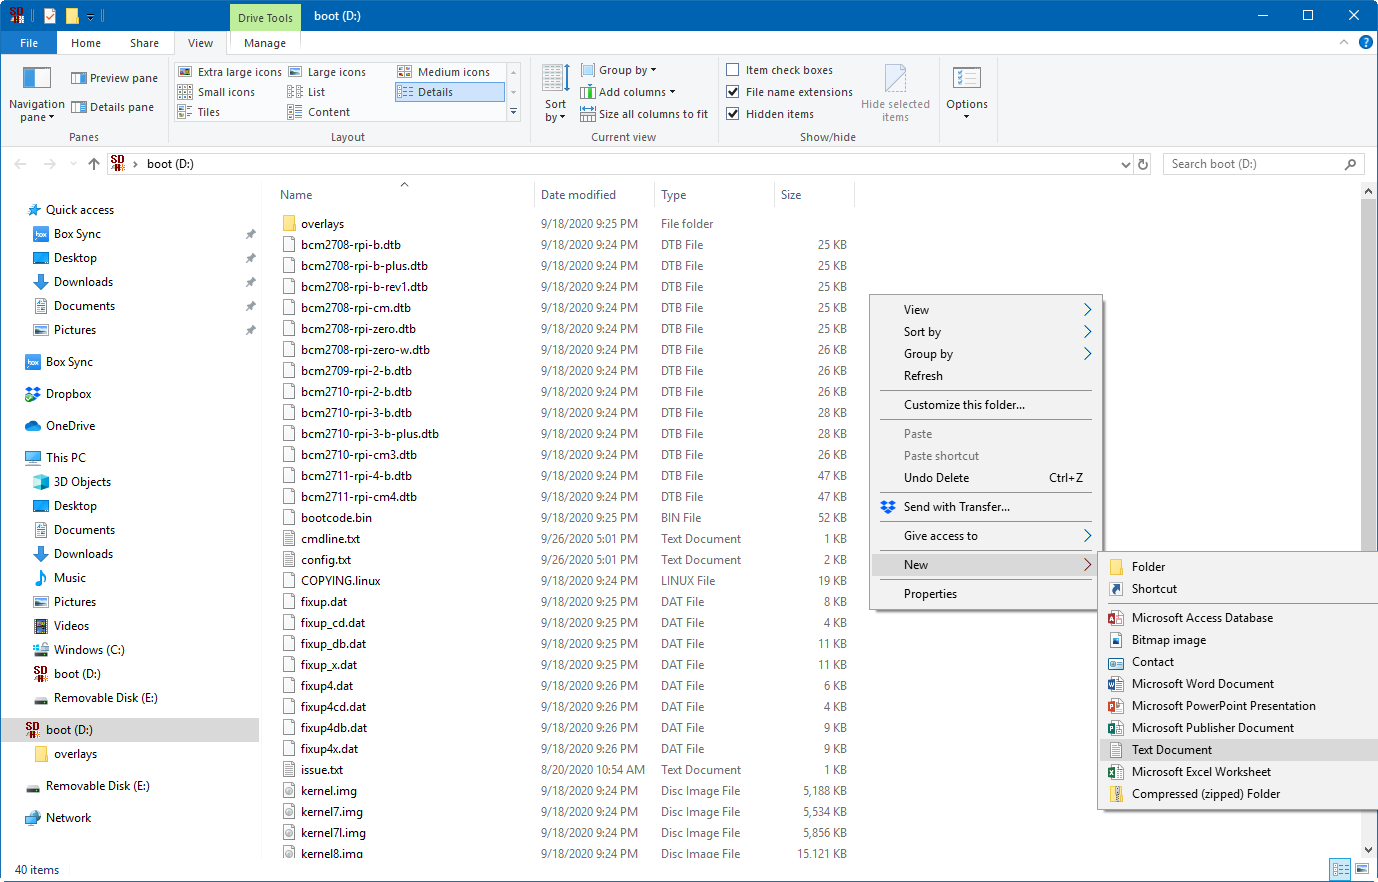
\includegraphics[width=1.00\textwidth]{sdbootnew}
\caption{Raspberry Pi Image Software. Use the program to select Raspberry Pi OS (Operating System) 32-bit. Then select the SD card location. Finally, click on ``Write''.}
\label{fig:pi_imager}
\end{figure}

  \item Registered Raspberry Pi with Pomona's network.
\end{enumerate}


\subsection{Update and Upgrading Raspberry Pi OS} 
\label{updateupgrade}

Every few months, the operating system should be updated. These have been updated on January 2025 with the following commands: 
\begin{enumerate}
\item First...!
 \begin{lstlisting}
  sudo apt update
  \end{lstlisting}
  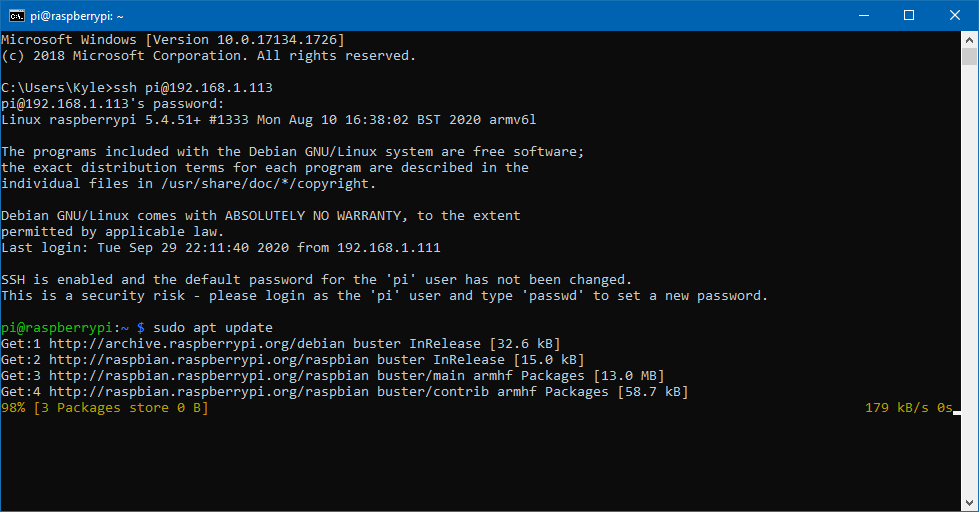
\includegraphics[width=1.00\textwidth]{aptupdate}
  \item Secondly, we want the Pi to compare the version list with its current packages and programs and update where needed. In your SSH session, type:
  \begin{lstlisting}
  sudo apt full-upgrade
  \end{lstlisting}
  \item You will be asked if you are sure you want to upgrade. Type \textbf{``y''} and \textbf{Enter}.
  \newline
  \newline
  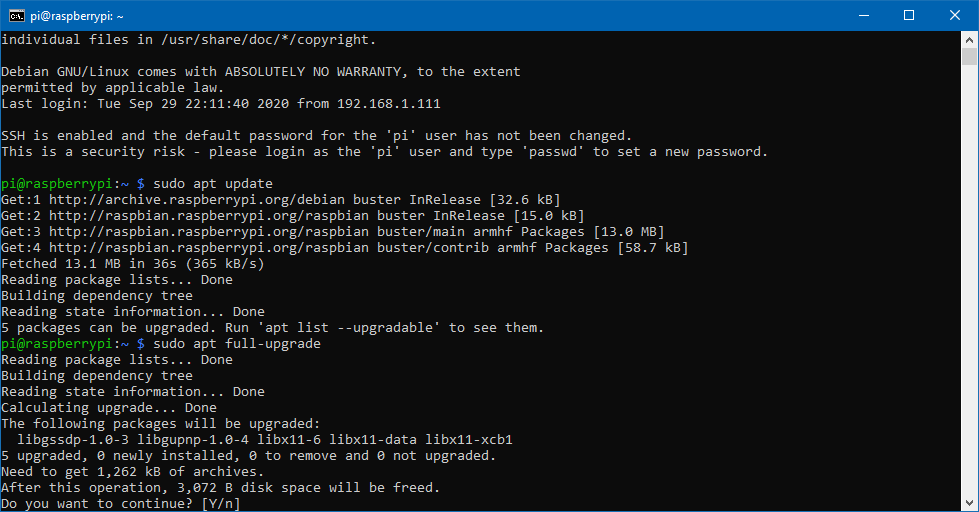
\includegraphics[width=1.00\textwidth]{aptupgradecont}
  \item Once it is finished, it will show this once again:
  \begin{lstlisting}
  pi@raspberrypi/:~ $_ 
  \end{lstlisting}
  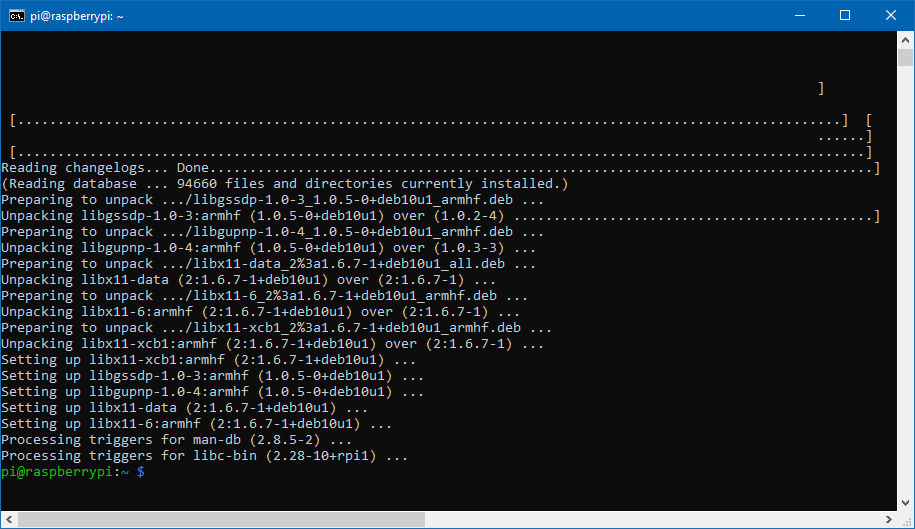
\includegraphics[width=1.00\textwidth]{aptupgradedone}
  \item Congratulations! Your Pi has been upgraded!
\end{enumerate}

\section{Configuring the Pi}

\subsection{Changing the Pi User Password??}

Note sure we will do this...

As a security measure, since your Pi is in your WiFi network, you'll want to change the password for the Pi.

\begin{enumerate}
  \item Run the Raspberry Pi configuration utility by using this command in the CLI:
  \begin{lstlisting}
  sudo raspi-config
  \end{lstlisting}
  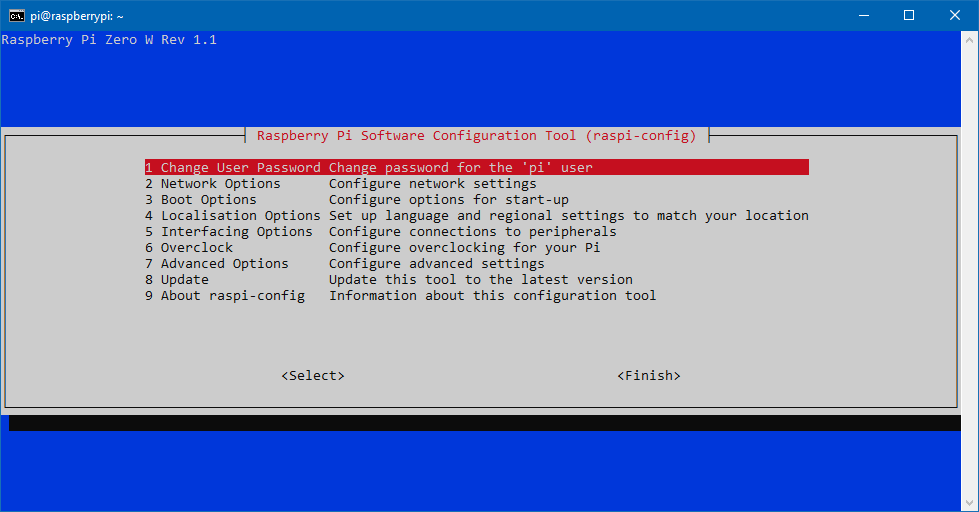
\includegraphics[width=1.00\textwidth]{rcpw}
  \item Navigate to \textbf{``Change User password for the 'pi' user''} and hit \textbf{Enter}.
  \item It will prompt you that it is going to ask for the new password. Press \textbf{Enter}, and type your new password followed by \textbf{Enter} again.
  \newline
  \newline
  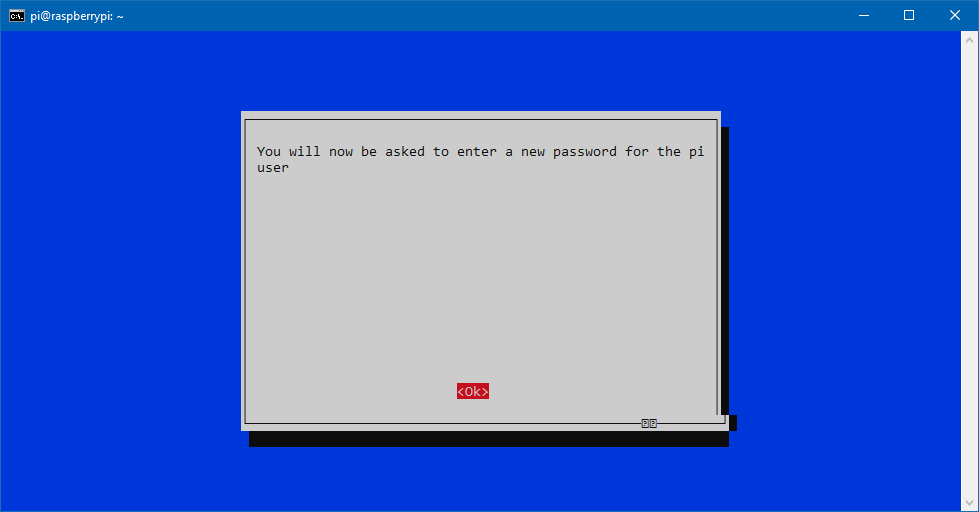
\includegraphics[width=1.00\textwidth]{rcpwconf}
  \item Verify the password by typing it again.
  \newline
  \newline
  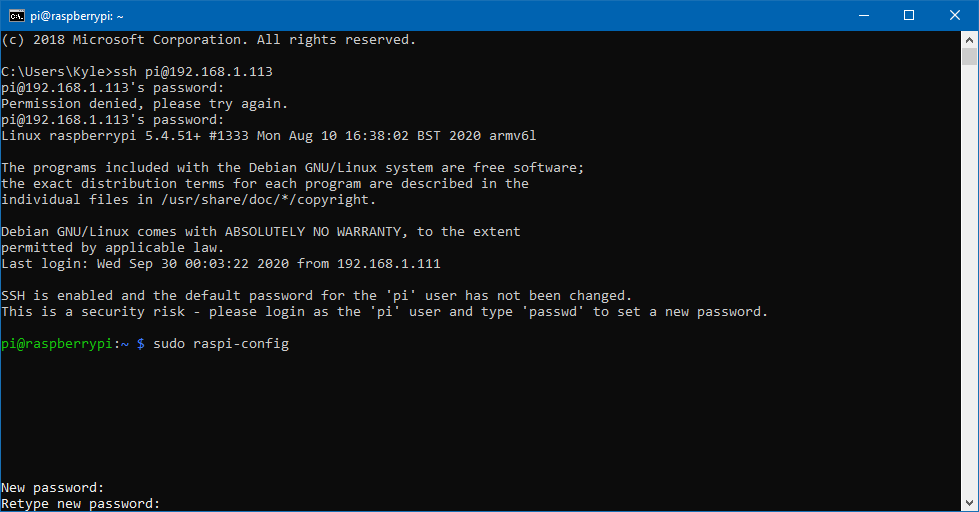
\includegraphics[width=1.00\textwidth]{rcpwretype}
  \item Your Pi now has your new password. Don't forget it!
\end{enumerate}

\subsection{Network Options}



\subsection{Virtual Network Computing (VNC) Option}

\textbf{NOTE} RealVNC lets you control the Pi via a graphical user interface (GUI)\url{https://www.youtube.com/watch?v=NWBmYnNvN3A}.

\begin{enumerate}
  \item While still in the raspi-config utility, navigate to \textbf{``Interfacing Options''}.
  \newline
  \newline
  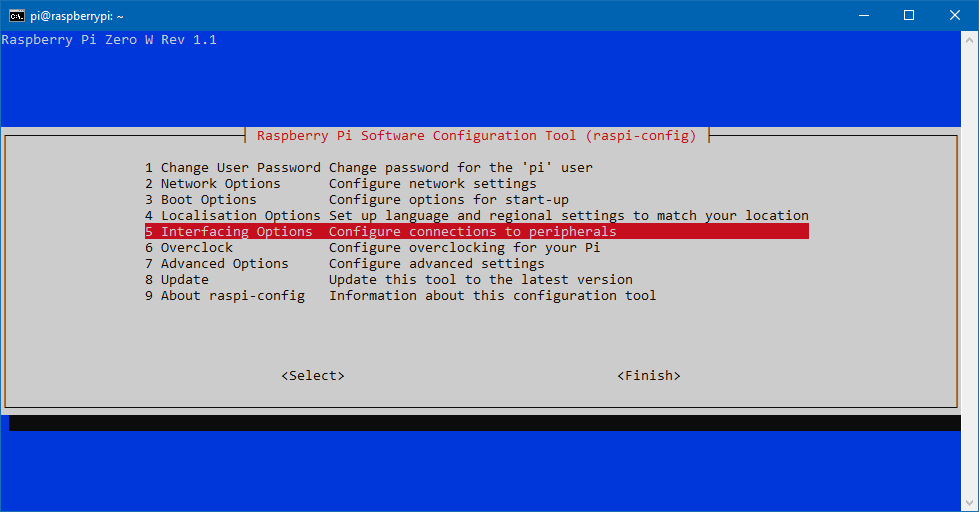
\includegraphics[width=1.00\textwidth]{rcifoptions}
  \item Navigate to \textbf{``VNC''} and select it.
  \newline
  \newline
  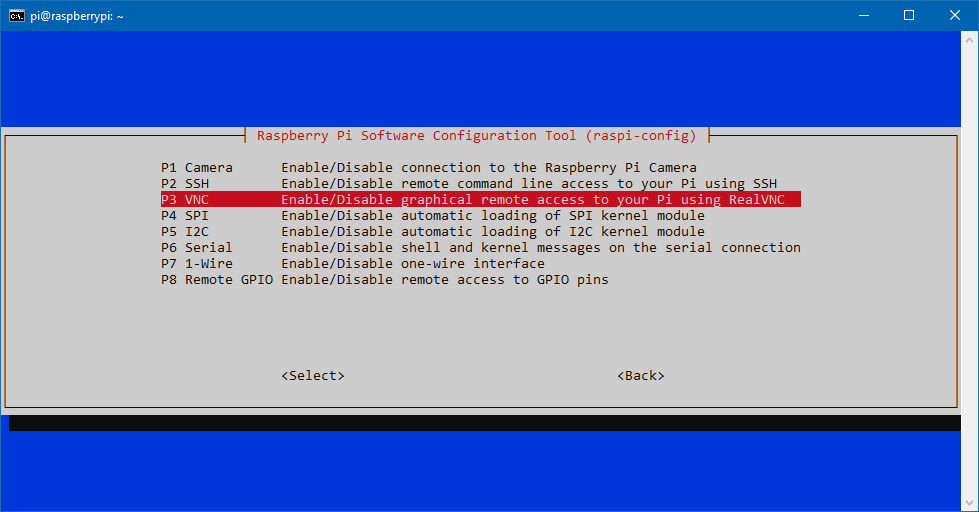
\includegraphics[width=1.00\textwidth]{rcvnc}
  \item The Pi will prompt you if you want the \textbf{VNC Server} enabled. Select \textbf{``Yes''}.
  \newline
  \newline
  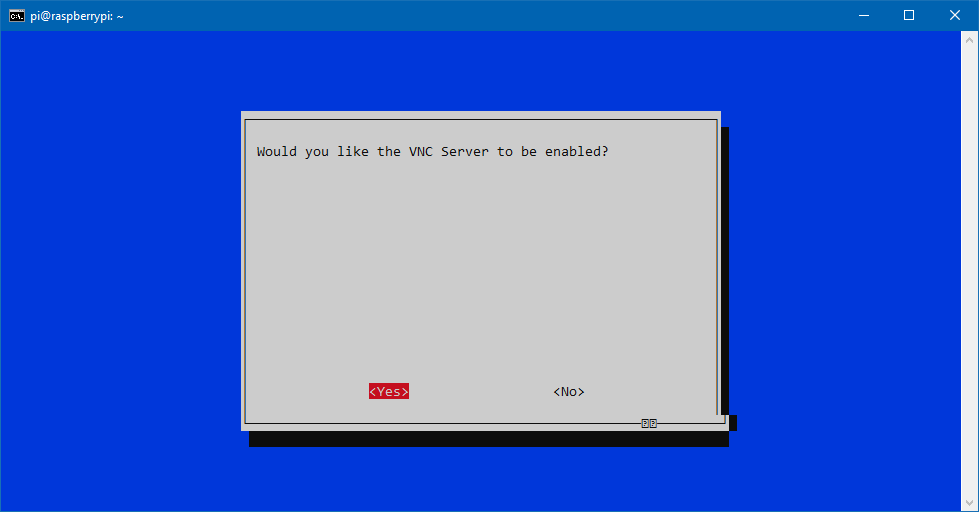
\includegraphics[width=1.00\textwidth]{rcvncenable}
  \item Wait a second and the Pi should let you know that the \textbf{VNC Server} is now enabled. This server will start automatically when the Pi boots up.
  \newline
  \newline
  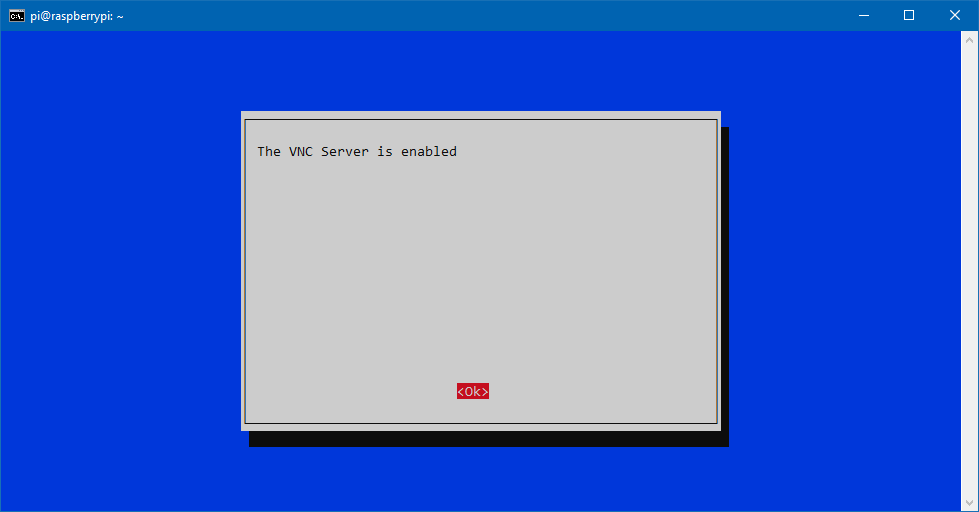
\includegraphics[width=1.00\textwidth]{rcvncconf}
  \item You still need to download \textbf{RealVNC} \textbf{\textit{Viewer}} on the computer you want to remotely access the Pi with.
  \item \textbf{RealVNC Viewer} can be downloaded at:
  \newline
  \url{https://www.realvnc.com/en/connect/download/viewer/}\footnote{I don't think this will work -- I prefer using remote desktop connection... why did you pick this one?} \footnote{Raspberry Pi OS comes with RealVNC Server already installed, you just have to enable the option (covered in the SOP). The other requirement is that you download RealVNC Viewer on the computer you want to VNC in with. I chose this route because it already is sort of equipped with RasPi OS, and the Viewer is cross-platform so I wouldn't need to write two sections of the SOP, on OSX and Windows.}
  \item Download the client that is for your OS and then install it.  
  \item When you open VNC Viewer, you should see something like the image below. In the top toolbar, input the IP address of the Pi and hit \textbf{``Enter''}.
  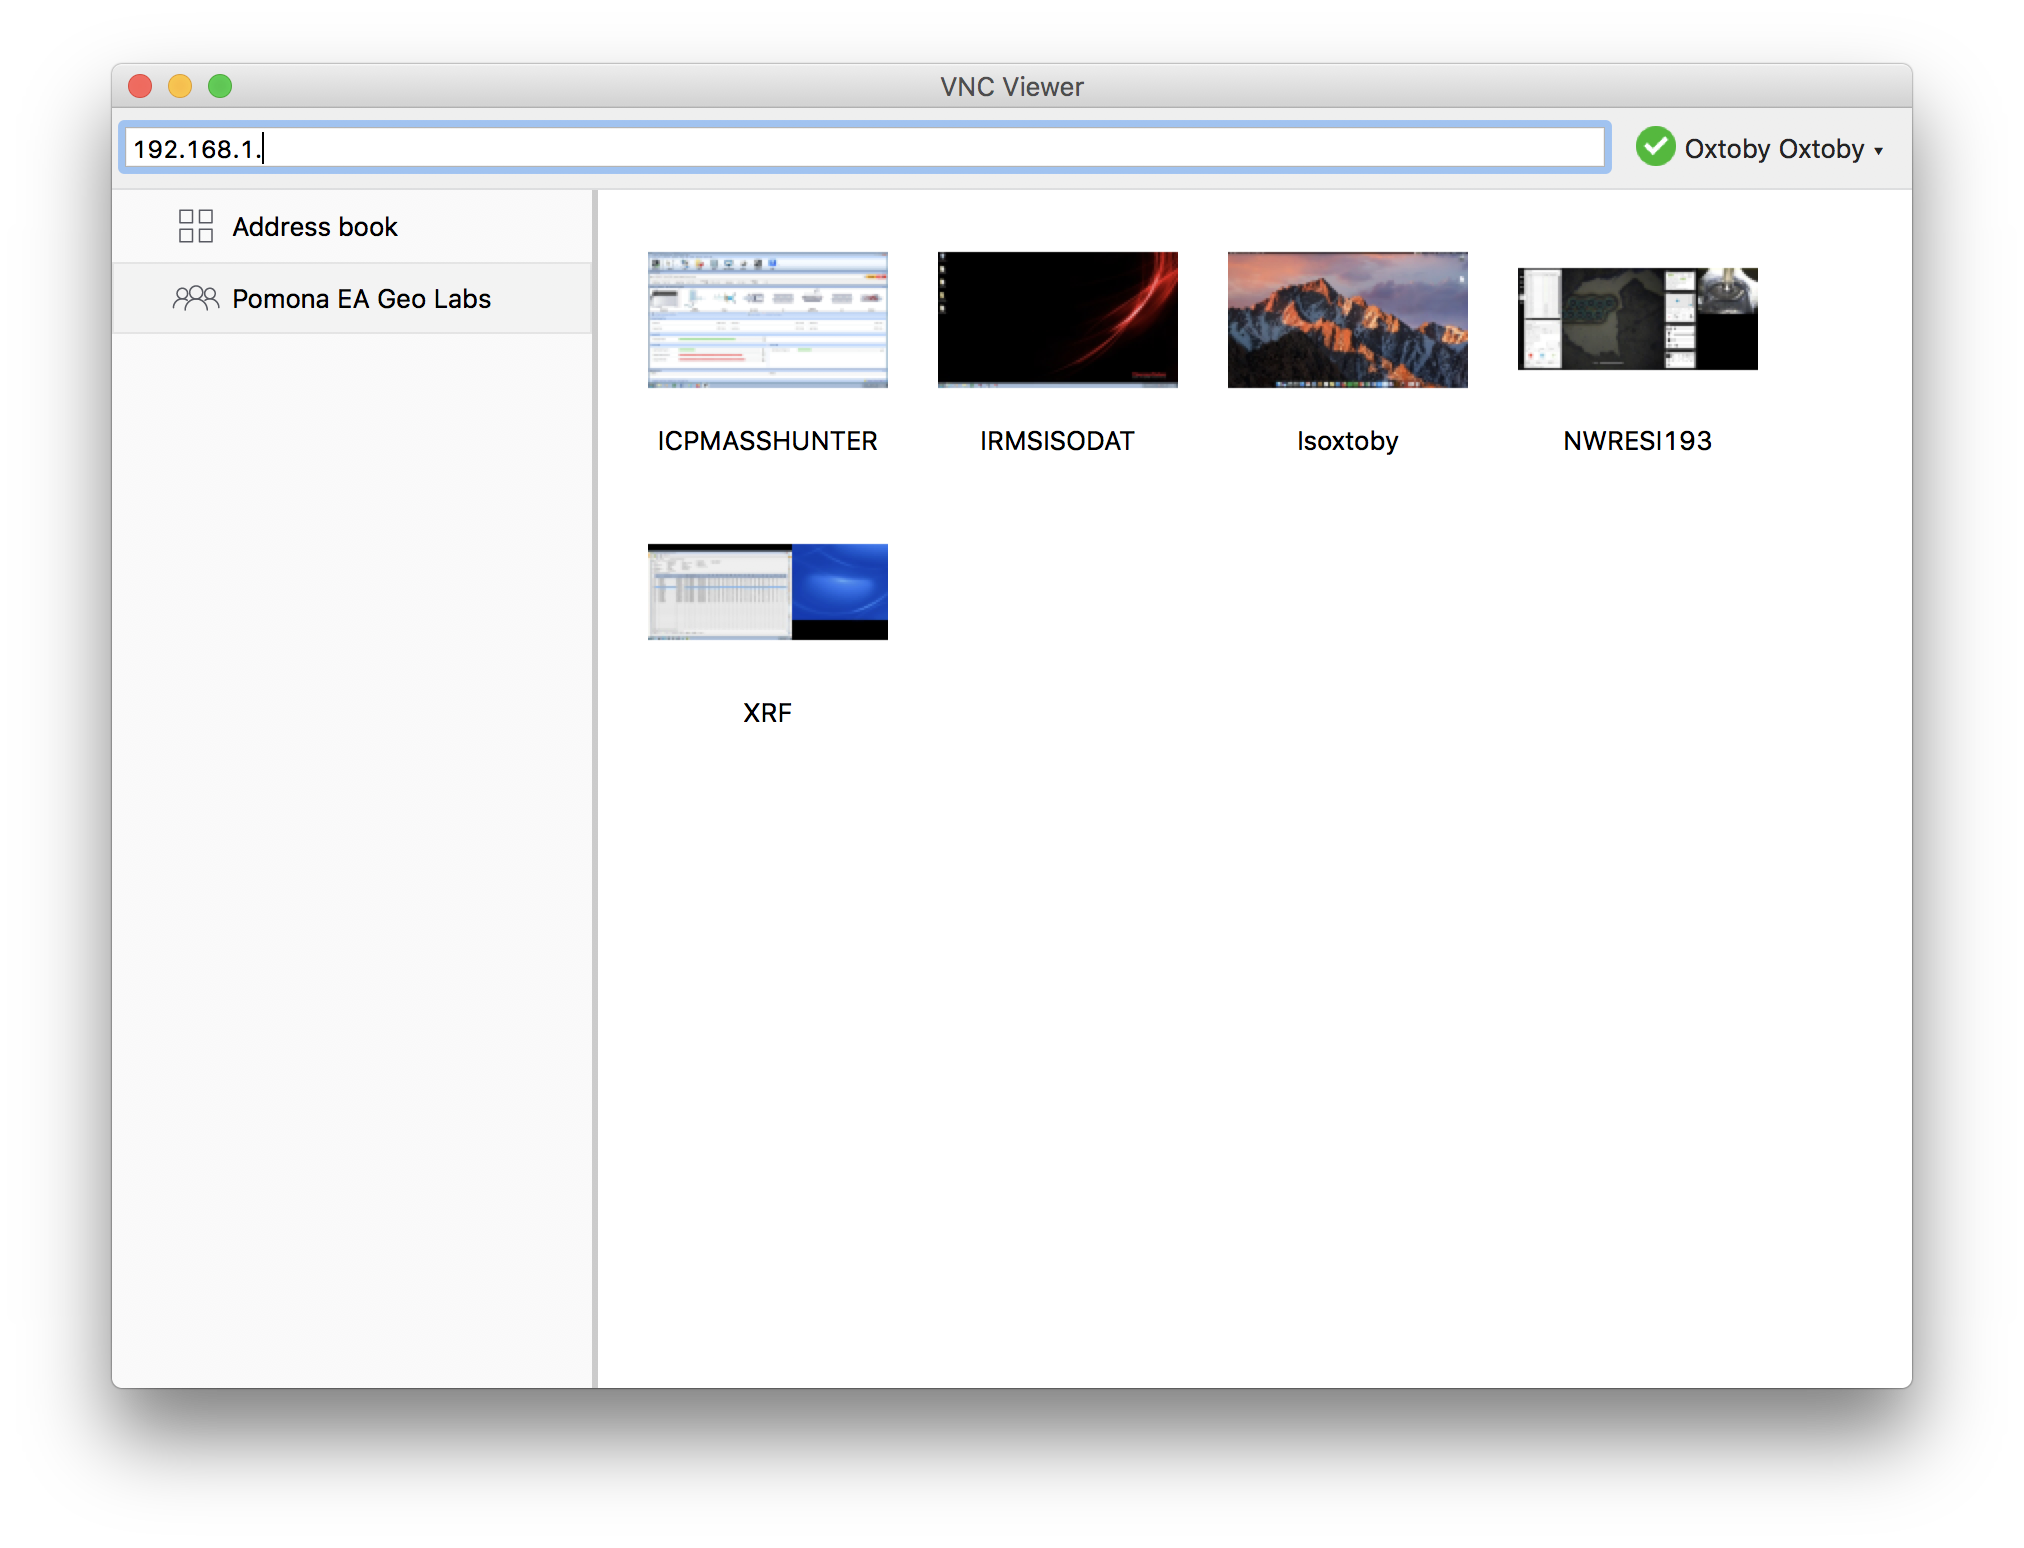
\includegraphics[width=1.00\textwidth]{realvnc}
  \item You will be prompts for the username (pi) and the password -- These are your pi's username and password. Remember changing your password will be a good idea a some point.
  \item Wait a minute and you should eventually see the desktop of the Pi. You can can browse and manipulate with your mouse etc.
\end{enumerate}

\section{Finishing Up}



\end{document}
